\section{Durchführung}
\label{sec:Durchführung}

\section{Durchführung}
Der Versuchsaufbau wird in \autoref{fig:1} dargestellt.
\begin{figure}[H]
  \centering
  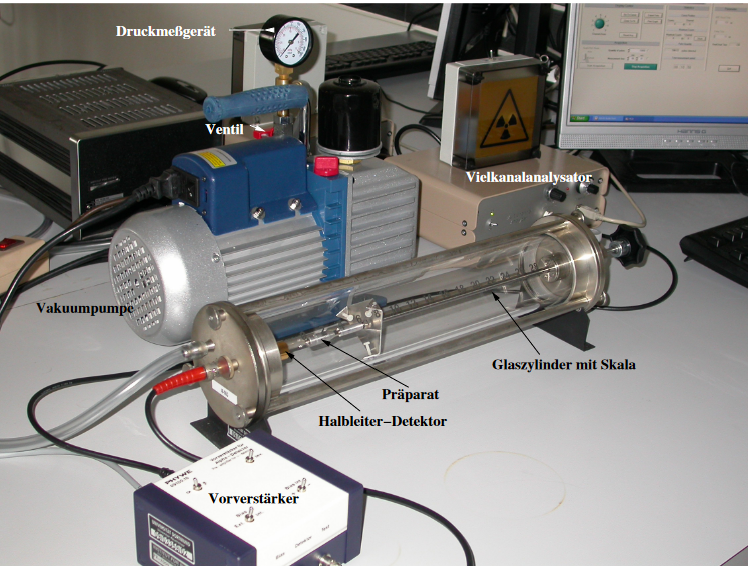
\includegraphics[width=9cm]{content/aufbau}
  \caption{Bild des Versuchsaufbaus.}
  \label{fig:1}
\end{figure} 
In dem evakuierbaren Glaszylinder befindet sich ein $\alpha$-Teilchen abstahlendes Am-Präparat mit Halbwertszeit $\textrm{T}_{1/2}=458$ a und ein Detektor. Der Abstand des Präparats zum Detektor ist variierbar. Der Detektor ist ein Halbleitersperrzähler und fällt ein Ion ein, bildet in der Verarmungszone des pn-Übergangs einen Stromimpuls, der durch einen OP-Verstärker analysierbar verstärkt wird. Vor der Messung sollte die Verkabelung überprüft werden, wobei der Sperrschichtzähler nur im spannungslosen Zustand verkabelt werden darf.

\subsection{Bestimmung der Reichweite von Alpha-Strahlung}
Zuerst wird der Glaszylinder evakuiert. Der Druck sollte dabei bei $p\approx 0$ liegen. Dann wird die Energieverteilung und die Zählrate der $\alpha$-Strahlung in Abhängigkeit vom Druck $p$ in Abständen von 50 mbar gemessen. Die Meßzeit beträgt 120 Sekunden. 

\subsection{Statistik des radioaktiven Zerfalls}
Für die Statistik des radioaktiven Zerfalls wird bei einem evakuierten Glaszylinder die Zerfälle pro Zeiteinheit mindestens 100 mal gemessen. Die Meßzeit beträgt 10 Sekunden. 
